\documentclass{assignment}

\class{SI 315}
\title{Assignment 1}
\author{Silas Falde}

\begin{document}
\maketitle
\tableofcontents

\section{Network 1}
\begin{figure}[h]
    \centering
    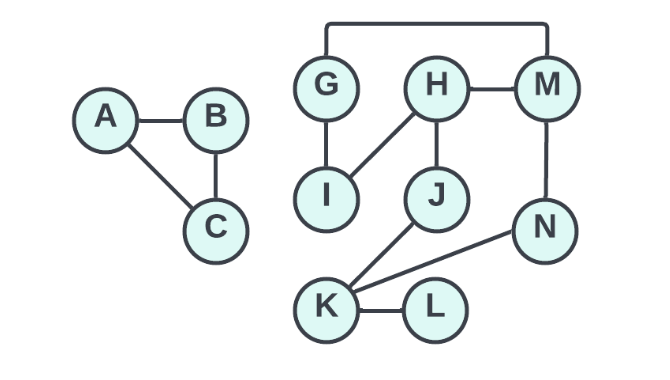
\includegraphics[width=0.5\textwidth]{figs/network-1.png}
    % List of connections (non-directional): 
    % component 1:
    % a to b, a to c
    % b to c
    % component 2: 
    % G to M, G to I
    % M to H, M to N
    % H to I, H to J
    % J to K
    % K to N
    % K to L
\end{figure}

\subsection{Longest Cycles}
\begin{problem}
    Identify the longest cycles in the network.
\end{problem}
The cycle $I \to G \to M \to N \to K \to J \to H \to I$ has 7 nodes and is the only longest cycle.

\subsection{Connectedness}
\begin{problem}
    Is the network connected? Explain.
\end{problem}

The network is not connected because there are nodes that cannot be reached from other nodes (e.g. $B \to I$).

\subsection{Connected Components}

\begin{problem}
    How many connected components does the network have? Which nodes are in each component?
\end{problem}

The network has two connected components:
\begin{itemize}
    \item Component 1: $A, B, C$
    \item Component 2: $G, M, N, K, L, J, H, I$
\end{itemize}

\subsection{Size of Connected Components}

\begin{problem}
    How many nodes are in the largest component of the network?
\end{problem}
The largest component is Component 2, which has 8 nodes: $G, M, N, K, L, J, H, I$.

\subsection{Breadth-First Search}
\begin{problem}
    Find the distance from node H to every other node in the network using breadth-first search. Draw a diagram of the breadth-first search procedure similar to the one shown in class, where each new layer of nodes is identified and circled. Remember, the BFS diagram should have all of the nodes in it!
\end{problem}

The breadth-first search layers starting at $H$ are:
\begin{itemize}
    \item Distance $0$: $H$
    \item Distance $1$: $I, J, M$
    \item Distance $2$: $G, K, N$
    \item Distance $3$: $L$
    \item Unreachable from $H$: $A, B, C$
\end{itemize}

% TODO: Draw the BFS diagram for the network starting at node H.

\subsection{Add One Edge}
\begin{problem}
    What is the longest cycle you can make by adding one edge to the network? Please specify what edge you would add, how long the longest resulting cycle is, and the cycle itself (i.e., the sequence of nodes). You do not have to explain how you found the edge and the cycle.
\end{problem}

The longest cycle can be made by adding the edge $C \to G$. The resulting longest cycle is $I \to G \to C \to A \to B \to C \to G \to M \to N \to K \to J \to H \to I$, which has 11 nodes.

\section{Network 2}

\begin{problem}
    In the network below, the ties (P, X), (P, Y), (Q, X), (Q, Y), (R, V), and (R, Z) are labeled strong (S), while all others are labeled weak (W).
\end{problem}

\begin{figure}[h]
    \centering
    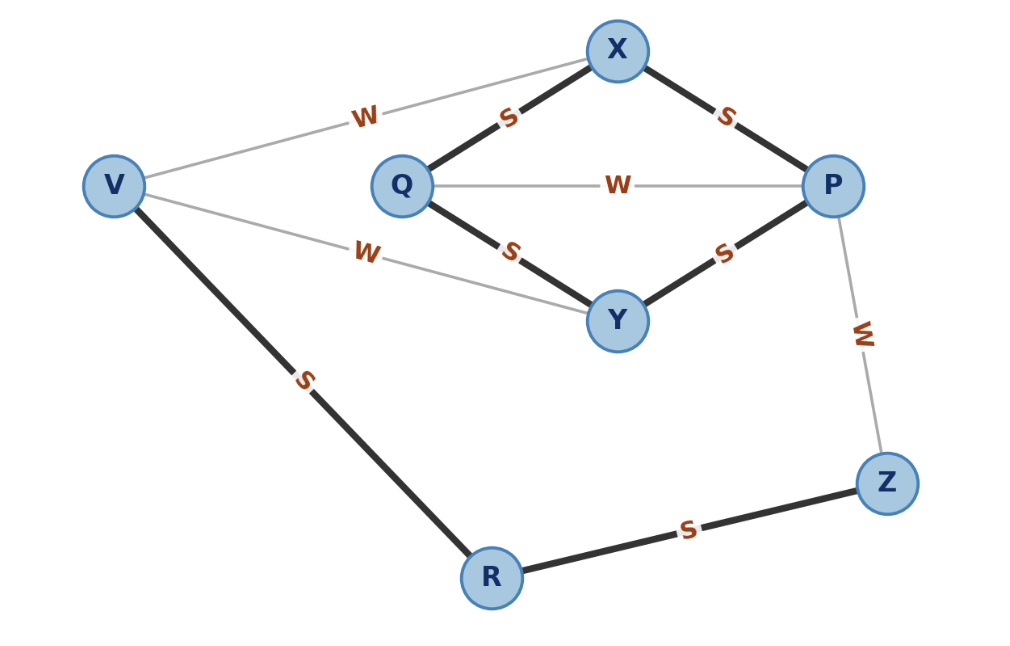
\includegraphics[width=0.8\textwidth]{figs/network-2.png}
    % Strong ties are labeled with (S) and weak ties with (W) in the figure.
    % Connections:
    % P to Q (W), X (S), Y (S), and Z (W)
    % Q to X (S), Y (S)
    % X to V (W)
    % Y to V (W)
    % Z to R (S)
    % V to R (S)
\end{figure}

\begin{problem}
    Identify all nodes that violate the Strong Triadic Closure Property. For each one, name its strong ties and the missing edge.
\end{problem}

\end{document}